\documentclass{article}  % Defines the type of document as an article

\usepackage{tikz}  % Imports the TikZ package for drawing diagrams

\usetikzlibrary{shapes.geometric, positioning}  % Imports specific TikZ libraries for shapes and positioning

\title{CS108\_LaTeX}  % Sets the title of the document

\author{Saksham Rathi}  % Sets the author(s) of the document

\date{March 2024}  % Sets the date of the document

\begin{document}  % Begins the document

\maketitle  % Creates the title page with the specified title, author, and date

\section{Diagrams}  % Starts a new section titled "Diagrams"

\subsection{Flowchart}  % Subsection titled "Flowchart"
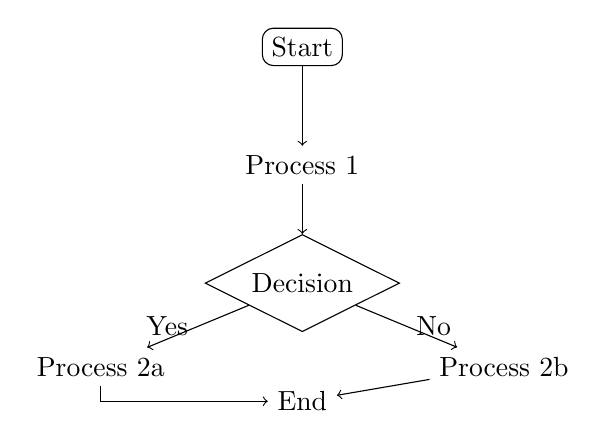
\begin{tikzpicture}[node distance=1.5cm]  % Begins a TikZ picture environment with specified node distance
    % Nodes
    \node (start) [draw, rounded corners] {Start};  % Defines a node named "start" with specified shape and text
    \node (process1) [below of=start] {Process 1};  % Defines a node named "process1" below the "start" node
    \node (decision) [below of=process1, diamond, aspect=2, draw] {Decision};  % Defines a diamond-shaped node named "decision" below the "process1" node
    \node (process2a) [below left of=decision, xshift=-1.5cm] {Process 2a};  % Defines a node named "process2a" below and to the left of the "decision" node
    \node (process2b) [below right of=decision, xshift=1.5cm] {Process 2b};  % Defines a node named "process2b" below and to the right of the "decision" node
    \node (end) [below of=decision] {End};  % Defines a node named "end" below the "decision" node
    
    % Arrows
    \draw [->] (start) -- (process1);  % Draws an arrow from "start" to "process1"
    \draw [->] (process1) -- (decision);  % Draws an arrow from "process1" to "decision"
    \draw [->] (decision) -- node[left] {Yes} (process2a);  % Draws an arrow from "decision" to "process2a" with a label "Yes"
    \draw [->] (decision) -- node[right] {No} (process2b);  % Draws an arrow from "decision" to "process2b" with a label "No"
    \draw [->] (process2a) |- (end);  % Draws an arrow from "process2a" to "end"
    \draw [->] (process2b) -- (end);  % Draws an arrow from "process2b" to "end"
\end{tikzpicture}

\subsection{Network Diagram}  % Subsection titled "Network Diagram"
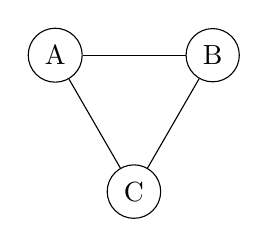
\begin{tikzpicture}  % Begins a TikZ picture environment
    % Nodes
    \node[circle,draw] (a) at (0,0) {A};  % Defines a circular node named "a" at coordinates (0,0) with text "A"
    \node[circle,draw] (b) at (2,0) {B};  % Defines a circular node named "b" at coordinates (2,0) with text "B"
    \node[circle,draw] (c) at (1,-1.732) {C};  % Defines a circular node named "c" at coordinates (1,-1.732) with text "C"
    
    % Connections
    \draw (a) -- (b);  % Draws a line connecting node "a" and node "b"
    \draw (b) -- (c);  % Draws a line connecting node "b" and node "c"
    \draw (c) -- (a);  % Draws a line connecting node "c" and node "a"
\end{tikzpicture}

\section{Graphs}  % Starts a new section titled "Graphs"

\subsection{Bar Chart}  % Subsection titled "Bar Chart"
\begin{tikzpicture}  % Begins a TikZ picture environment
    \draw (0,0) rectangle (1,2);  % Draws a rectangle at specified coordinates
    \draw (1.5,0) rectangle (2.5,3);  % Draws a rectangle at specified coordinates
    \draw (3,0) rectangle (4,1.5);  % Draws a rectangle at specified coordinates
\end{tikzpicture}

\subsection{Pie Chart}  % Subsection titled "Pie Chart"
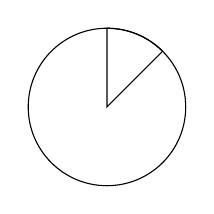
\begin{tikzpicture}  % Begins a TikZ picture environment
    \draw (0,0) circle (1);  % Draws a circle with specified radius and center
    \draw (0,0) -- (45:1) arc (45:90:1) -- cycle;  % Draws an arc of a circle
\end{tikzpicture}

\subsection{Scatter Plot}  % Subsection titled "Scatter Plot"
\begin{tikzpicture}  % Begins a TikZ picture environment
    \draw[<->] (0,4) node[left]{$y$} -- (0,0) -- (4,0) node[below]{$x$};  % Draws axes with labels
    \draw (0.5,1) node[circle,fill,inner sep=1.5pt]{}  % Draws a filled circle at specified coordinates
          (1,2) node[circle,fill,inner sep=1.5pt]{}  % Draws a filled circle at specified coordinates
          (1.5,3) node[circle,fill,inner sep=1.5pt]{};  % Draws a filled circle at specified coordinates
\end{tikzpicture}

\section{Mathematical Illustrations}  % Starts a new section titled "Mathematical Illustrations"

\subsection{Function Plot}  % Subsection titled "Function Plot"
\begin{tikzpicture}  % Begins a TikZ picture environment
    \draw[<->] (-2,0) -- (2,0) node[right]{$x$};  % Draws x-axis with label
    \draw[<->] (0,-1) -- (0,2) node[above]{$y$};  % Draws y-axis with label
    \draw[color=blue,domain=-1.5:1.5] plot (\x,{\x^2});  % Plots a function
\end{tikzpicture}

\subsection{Geometry}  % Subsection titled "Geometry"
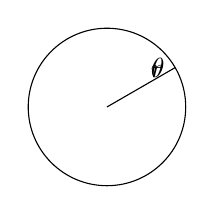
\begin{tikzpicture}  % Begins a TikZ picture environment
    \draw (0,0) circle (1);  % Draws a circle with specified radius and center
    \draw (0,0) -- (30:1) node[midway,above right]{$r$};  % Draws a line and labels the midpoint
    \draw (30:0.5) node[above right]{$\theta$};  % Labels a point
\end{tikzpicture}

\section{Animations}  % Starts a new section titled "Animations"

\subsection{Animating Circles}  % Subsection titled "Animating Circles"
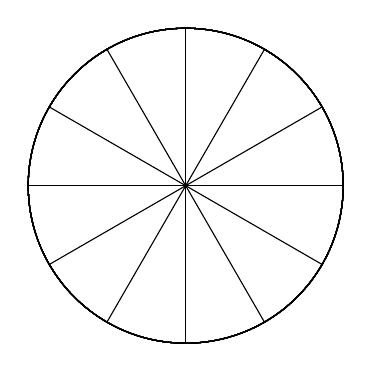
\begin{tikzpicture}[scale=2]  % Begins a TikZ picture environment with specified scale
    \foreach \x in {0,30,...,360} {  % Loops through angles
        \draw (0,0) circle (1);  % Draws a circle with specified radius and center
        \draw (0,0) -- (\x:1);  % Draws a line at the specified angle
    }
\end{tikzpicture}

\end{document}  % Ends the document
